% IH-214 full article in English, laid out with the AERO2027 abstract template styles.
% DRAFT: not approved for submission. Pending items are marked \pendente{...} in red.
%
% Format assumption (stated, not given by the event): AERO2027 asks only for a one-page
% abstract (deliverables/EVENTO_AERO2027.md). This full article reuses the template's
% typography and section order (Title, Authors, Abstract, Keywords, [body], References,
% Biography): Times, title 14 pt bold centred, authors 12 pt, affiliations 11 pt italic,
% text 12 pt justified with Word-equivalent 1.5 line spacing, A4, 2.54 cm margins.
%
% Evidence sources (every number below comes from these archived files, D4.1 v2.2,
% code 1262bb2): data/d4/resumo_celulas_d4_5.csv, data/d4/contrastes_d4_5.csv,
% data/d4/sintese_d4_5.md, data/d4/traco_d4_6.md; model inputs in
% data/parameter_registry.csv and data/model_dictionary.csv; literature claims in
% data/d3/extracao.md and data/d3/sintese_mecanismos.md.
% References are generated from references/references.bib by gerar_referencias.py.
%
% Build: python gerar_referencias.py artigo_aero2027_en.tex ../../references/references.bib referencias_aero.tex
%        pdflatex artigo_aero2027_en (twice)

\documentclass[12pt,a4paper]{article}
\usepackage[T1]{fontenc}
\usepackage[utf8]{inputenc}
\usepackage{mathptmx}                       % Times
\usepackage[margin=2.54cm]{geometry}
\usepackage{xcolor}
\usepackage[normalem]{ulem}
\usepackage{amsmath}
\usepackage{graphicx}
\usepackage{booktabs}
\usepackage{array}
\usepackage{caption}
\usepackage[hidelinks]{hyperref}
\usepackage{xurl}

\graphicspath{{../../figures/}{figures/}}   % local build or Overleaf root
\newcommand{\pendente}[1]{\textcolor{red}{[#1]}}
\linespread{1.428}                          % 12 pt Times at Word "1.5 lines" (20.7 pt)
\captionsetup{font={small,stretch=0.75},labelfont=bf}
\setlength{\parindent}{0pt}
\setlength{\parskip}{6pt}
\makeatletter
\renewcommand\section{\@startsection{section}{1}{\z@}{12pt}{4pt}{\fontsize{14}{20}\selectfont\bfseries}}
\renewcommand\subsection{\@startsection{subsection}{2}{\z@}{8pt}{2pt}{\normalsize\bfseries}}
\renewcommand\@biblabel[1]{[#1]}
\renewenvironment{thebibliography}[1]{%
  \section*{References}%
  \list{\@biblabel{\@arabic\c@enumiv}}{\settowidth\labelwidth{\@biblabel{#1}}%
    \leftmargin\labelwidth \advance\leftmargin\labelsep \usecounter{enumiv}%
    \itemsep 0pt \parsep 0pt}}{\endlist}
\makeatother
\pagestyle{plain}

\begin{document}

\begin{center}
\textcolor{red}{\small DRAFT: not approved by the authors for submission}\par\medskip
{\fontsize{14}{20}\selectfont\bfseries
Coupling Terminal Station Queues And Stand Retention At Vertiports:\\
A Paired Simulation Of Admission Policy And Resource Capacity\par}
\medskip
{\fontsize{12}{18}\selectfont
\uline{L. H. Tozi}\textsuperscript{1,*}, \pendente{co-authors and advisor}\textsuperscript{1}\par}
{\fontsize{11}{16}\selectfont\itshape
\textsuperscript{1}Instituto Tecnológico de Aeronáutica (ITA), \pendente{address}, Brazil.\par
\textsuperscript{*}\pendente{e-mail of the corresponding author}\par}
\end{center}

\section*{Abstract}
A vertiport operator with room for one more resource must choose between another stand and
another check-in counter, and must decide whether to admit flights in advance or first-come,
first-served (FCFS). Airside models schedule pads and stands, terminal models size passenger
stations without the airside, and coupled models report aggregate passenger delay rather than
queues at each station. We built a discrete-event simulation of a generic vertiport with one
TLOF, a shared taxi route and five stands. Charging and individual boarding are synchronised with
check-in, carry-on baggage and security queues, and both decisions are compared over 30 paired 8-h
synthetic days. At 6 requests/h with 30-min charging, a fifth stand added 0.487
passenger departures/h under FCFS (95\% CI: 0.439--0.536) and 0.492 under advance admission
(0.440--0.544). A second counter cut mean check-in waiting by 141.5~s under FCFS (124.7--158.4)
and raised compliance with the IATA 180-s waiting limit from 68\% to 99\%; 124.7~s (107.9--141.5)
of that waiting reappeared in the lounge, because boarding still waited for the charging aircraft.
Advance admission stayed within 0.033 departures/h of FCFS (0.001--0.066 fewer). Exploratory
families show that the stand pays off as demand and charging time grow, whereas the counter pays
off most when stands turn quickly. Inputs come from the literature or are stated assumptions, so
the results compare designs rather than predict a site.

{\itshape\textbf{Keywords:} Vertiport; Urban Air Mobility; Discrete-Event Simulation; Passenger
Processing; Admission Policy; Level of Service\par}

% ---------------------------------------------------------------------------------------
\section{Introduction}

Electric vertical take-off and landing (eVTOL) services will depend on vertiports whose
footprint is small and whose resources are expensive to add. Two decisions recur in their
design and operation. The first concerns capacity: whether a scarce increment of space or budget
should buy another aircraft stand or another passenger-processing server. The second concerns
coordination: whether arrival requests are admitted in advance against a resource schedule, as in
the reservation-based concept of operations described for high-density automated vertiports
\cite{kunchulia2021}, or served first-come, first-served when the aircraft asks for the
resources. Both decisions act on two populations at once. Stands and admission rules shape how
many aircraft depart, and counters and security posts shape how long passengers wait. The stand
links the two: an aircraft cannot leave before its passengers board, and passengers cannot board
before the aircraft is ready.

Existing studies examine these pieces with different boundaries. On the airside, Guerreiro et
al.\ \cite{guerreiro2020} reserve vertipad and parking timelines under an FCFS scheduler and find
configurations limited by pads and others by parking. Escribano Macias et al.\
\cite{escribanoMacias2023} size landing, charging, parking and take-off pads from the queueing of
aircraft, and Onat et al.\ \cite{onat2026buffer} show that a full parking area blocks the TLOF for
new arrivals. On the terminal side, Feldhoff \cite{feldhoff2022} simulates passenger processing
and evaluates waiting against IATA level-of-service limits without modelling the airside. Preis
and Hornung \cite{preisHornung2022,preisHornung2022heuristic} couple pad and gate operations to
passenger delay, but measure that delay as aggregate time on the airfield rather than as queues
at individual stations. Halder and Gandhi \cite{halderGandhi2025} compare FCFS with rule-based
departure sequencing under fixed infrastructure and report completed flights and fleet idle
time, not terminal queues.

This study targets the junction these works leave open: queues at each terminal station,
synchronised with group readiness, charging and stand retention, observed on both sides under
controlled contrasts. We make three contributions. First, we provide a verified discrete-event
model that couples a single-TLOF, multi-stand airside to three mandatory passenger stations and
individual boarding, with requests, manifests and service times generated before any policy acts.
Second, we estimate, with paired replications and pre-declared primary indicators, the effects of
a fifth stand, a second check-in counter and advance admission. Third, we show where the waiting
removed from one station goes, and under which demand and charging conditions each resource
increment pays off.

Section~\ref{sec:background} sets out the queueing mechanisms. Section~\ref{sec:method}
describes the model and the experiment, and Section~\ref{sec:verification} the verification.
Section~\ref{sec:results} reports the results, Section~\ref{sec:discussion} discusses their
operational meaning and scope, and Section~\ref{sec:conclusion} concludes.

% ---------------------------------------------------------------------------------------
\section{Queueing Mechanisms At A Passenger Vertiport}
\label{sec:background}

A vertiport queue can have an aircraft requesting a pad or a passenger arriving at check-in as
its unit, and that choice fixes what ``waiting'' means. For a stable queue, Little's law
$L=\lambda W$ relates the mean number of units present, the rate at which units are admitted
across a boundary and their mean time inside it \cite{little1961}. Applied to the queue in front
of a station, the time ends when service starts; applied to the whole station, it ends when the
passenger leaves. Our experiment uses a terminating 8-h window rather than a stationary regime,
so we report waits with their populations and censoring instead of inferring one quantity from
the other.

On the airside, the number of stands limits how many aircraft can be served at once, while the
observed throughput is the number of movements per hour. A practical capacity also requires a declared
delay criterion. Zhang et al.\ \cite{zhang2023capacity} obtain 53.3 or 31.9 sorties/h for the same
vertiport depending on whether 90~s or 30~s of delay is acceptable, and Preis and Hornung
\cite{preisHornung2022heuristic} define practical capacity by a threshold of mean delay. We therefore treat stand counts as inputs and departures per hour as outputs, and we
do not report a capacity. The FCFS scheduler of Guerreiro et al.\ \cite{guerreiro2020} also
reserves resources on timelines after each request, so a reservation is a data structure rather
than a policy. The policy contrast here is whether a request is admitted in advance against future
resource availability.

The stand connects the aircraft queue to passenger processing. The concept of operations of
NUAIR and NASA ties gate opening to aircraft readiness \cite{kunchulia2021}, and boarding in turn
depends on the passengers who will fly \cite{saxena2025vertiminal}. Converting movements into
passengers per hour requires seat occupancy and the sequence of individual service; Preis
\cite{preis2023} computes such flows under explicit occupancy and concurrency assumptions. In our
model, declared charging ends before passengers access the aircraft, and the stand is released
only after charging and after the last confirmed passenger has completed every mandatory station.
An additional stand lets the vertiport accept another aircraft while the others charge or wait
for passengers, without changing the terminal queues. An additional counter acts on group
readiness instead. Feldhoff \cite{feldhoff2022} observed, without an airside, that a second counter
reduces counter waiting, and attributed the low waiting downstream to the delay created at the
counter. Our hypothesis was that a second counter would advance boarding when the group retains
the aircraft and, when the aircraft is still charging, would merely move the waiting to the
lounge or to the next station.

Evaluating service requires knowing where and for whom the waiting occurs. Feldhoff
\cite{feldhoff2022} separates total processing time from the share of passengers whose wait
exceeds the limit of each station; we adopt the IATA limits she reproduces in her Table~5, not
the limits she adapts for air taxis in Table~6. Bennaceur et al.\ \cite{bennaceur2022} use the
expected wait between the planned arrival at the vertiport and the scheduled departure. We keep
both views with explicit start and end events. The temporal level of service is the share of
observed station waits within the station limit, and the wait from the end of security to the
start of boarding captures the delay after processing. Perceived satisfaction would require a
measure declared by passengers and is outside this study.

% ---------------------------------------------------------------------------------------
\section{Model And Experimental Design}
\label{sec:method}

\subsection{Boundary, resources and events}

The unit of analysis is a generic passenger vertiport during a finite 8-h window that opens with
free resources and empty queues. The airside follows the modular composition of the EASA
prototype technical specification \cite{easa2022ptsvptdsn} with one FATO--TLOF, one bidirectional
taxi route and four or five stands; the five-stand topology is the one Feldhoff
\cite{feldhoff2022} adopts from Vascik and Hansman \cite{vascikHansman2019}. We transfer the
topology, not the efficiency conclusion of that source. Each stand has its own charger and
passenger gate, an assumption that keeps a third bottleneck out of the questions studied. The
reference aircraft class is a piloted four-passenger eVTOL; flight, airspace routing and mission
energy are outside the boundary.

Each aircraft lands on the TLOF, is towed along the route to a stand and deboards one arriving
passenger. It then charges for the declared time, boards its confirmed passengers one by one in
the order they become ready, and returns along the route to the TLOF for take-off. TLOF possession, physical
occupation and post-exit separation are recorded as distinct intervals. Each passenger who shows
up passes check-in, carry-on baggage check and security, in that order, through single FCFS
queues without abandonment, and then waits in the lounge. When a station has two servers, the
first passenger in line takes the first free server. Table~\ref{tab:inputs} lists the inputs and
their provenance.

\begin{table}[htbp]
\centering\small
\caption{Model inputs and their nature. Durations from expert-based sources are used as
constants; values marked ``author'' are scenario assumptions.}
\label{tab:inputs}
\renewcommand{\arraystretch}{0.9}
\begin{tabular}{@{}>{\raggedright\arraybackslash}p{0.43\linewidth}>{\raggedright\arraybackslash}p{0.2\linewidth}>{\raggedright\arraybackslash}p{0.3\linewidth}@{}}
\toprule
Input & Value & Source \\
\midrule
Touchdown to TLOF exit (towed); separation & 37.7 s; 3 s & author distances, \cite{preisHornung2022}; author \\
Taxi per route leg & 22.8 s & author distances, \cite{preisHornung2022,wille2024icas} \\
Tow removal, deboarding, gate exit & 27; 65.8; 26.7 s & \cite{preisHornung2022} \\
Walk, aircraft access, boarding per passenger & 31.9; 19.7; 73.0 s & \cite{preisHornung2022} \\
Tow attachment; departure TLOF occupation & 27 s; 50 s & \cite{preisHornung2022}; author \\
Declared charging per turnaround & 0, 30 or 60 min & \cite{preis2023} \\
Check-in; security (deterministic) & 180 s; 90 s & author \\
Carry-on baggage check & U(30, 60) s & \cite{feldhoffSoaresRoque2021} \\
Passenger arrival before scheduled departure & 15--60 min, uniform & window \cite{feldhoff2022}; shape author \\
Reservations per request; no-show probability & 1--4; 0.10 & author \\
Station waiting limits (counter, security) & 180 s; 180 s & IATA via \cite{feldhoff2022} \\
\bottomrule
\end{tabular}
\end{table}

\subsection{Offered demand}

Each replication is one synthetic day generated before any policy acts, so that every cell of a
replication receives the same requests, manifests, arrivals and service times. Aircraft requests
follow a homogeneous Poisson process at 8 requests/h from 2,700~s to the end of the window. Each
request carries an independent uniform mark; the 6 and 4 requests/h families keep the requests
whose mark falls below 0.75 and 0.5, respectively, so the lower-demand days are nested subsets of
the higher-demand one. A request issued at time $t$ has a scheduled departure
$\mathrm{STD}=t+900~\text{s}+R$, where $R$ is the declared charging time, and its manifest closes
900~s before the STD. Passengers who show up arrive between 60 and 15~min before the STD; the
window comes from Feldhoff \cite{feldhoff2022}, while the uniform shape is our assumption because
the source does not publish the parameters of its beta distribution. A group with nobody present
at manifest closure is cancelled if its aircraft has not yet been allocated; an aircraft already
admitted completes its cycle and departs empty, and such departures are reported separately.

\subsection{Policies}

Under FCFS, each resource serves the oldest eligible request. An arriving aircraft needs the TLOF,
the route and a stand at the same time; if it cannot start its approach within 300~s of the
request, it diverts and its passengers are notified at that instant. Under advance admission, the
request is decided at $t$. The scheduler builds the calendar of admitted commitments, with an
updated forecast for each flight, and looks for the first feasible touchdown in $[t, t+300~\text{s}]$
on the lowest-index stand that fits. If none fits, it refuses the request and notifies the
passengers at $t$. The forecast of group readiness uses the observed queues and declared service times for
passengers already in the terminal and assumes that passengers not yet arrived will arrive at
manifest closure, the latest arrival compatible with the rules. No decision uses future requests.

During execution, touchdown does not precede its planned time, but the planned stand exit is a
priority rather than a minimum time. An aircraft ready before its plan leaves as soon as the route
and the TLOF are free, and later decisions use the updated forecast. This mirrors the renegotiation
of a reservation that is compatible with the resource plan in the NASA concept of operations
\cite{kunchulia2021}, which describes arrival reservations; applying it to departures is our
assumption. Passengers notified of a refusal or diversion leave the queue at once, finish a service
already under way, or leave the lounge.

\subsection{Configurations, families and indicators}

Three configurations share one TLOF, one route, one baggage station and one security post:
Base (five stands, one counter), S4 (four stands) and B2 (five stands, two counters). Each runs
under both policies. Five families vary one factor from the reference (6 requests/h, 30-min
charging): 4 and 8 requests/h, and 0 and 60~min of charging. Two further families give the
scheduler perfect information about arrivals and baggage durations, with 30 and 0~min of
charging, and reuse the FCFS cells of their control families. Each replication thus has 36
distinct cells. Because counter and security services are deterministic and security is faster
than check-in, successive arrivals at security are at least 150~s apart with one counter, so no
security queue forms; we therefore did not run a second security post.

Throughput $X$ counts departures carrying passengers within the window, divided by its 8~h. For
station $j$, the individual wait is $W_{ij}=t^{\mathrm{start}}_{ij}-t^{\mathrm{entry}}_{ij}$, and
the temporal level of service is
\begin{equation}
 C_j=\frac{1}{|O_j|}\sum_{i\in O_j}\mathbf{1}\!\left(W_{ij}\leq \tau_j\right),
\end{equation}
where $O_j$ contains the visits whose service start was observed and $\tau_j$ is the station
limit; waits still open at the horizon are censored and reported apart. The post-security wait
runs from the end of security to the start of the passenger's own boarding and includes 51.6~s of
walking and aircraft access. Group retention is the time a ready aircraft waits for its
passengers, and stand blocking is the time between departure readiness and stand exit. Request
outcomes are closed as cancelled, refused, diverted, departed or pending at the horizon.

\subsection{Statistical design}

Before the runs, we fixed one primary indicator per contrast in the reference family: passenger
departures/h for advance admission minus FCFS (Base) and for Base minus S4 (each policy), and mean
counter waiting for B2 minus Base (each policy). All other contrasts and families are exploratory.
A pilot with 30 independent days (seeds 10001--10030) estimated the dispersion of the paired
differences; the largest estimated requirement was 11 replications, below the pre-set minimum of
30, so the definitive runs used 30 new days (seeds 20001--20030). Each effect is computed within
the replication and summarised by its mean and a two-sided 95\% $t$ interval, following the paired
design described by Law \cite{law2023design}. Proportions are means of per-replication ratios.

% ---------------------------------------------------------------------------------------
\section{Verification}
\label{sec:verification}

The simulator was built in four verified phases: TLOF mutual exclusion and separation; route and
stand; turnaround decomposition and charging; and the terminal with manifests, three stations,
boarding and service metrics. Hand-computed cases check simultaneous requests, route and stand
blocking, zero and positive charging, a wait exactly at the 180-s limit and incomplete groups. They
also check the inclusive 300-s window (touchdown allowed at $t+300$~s, diversion at $t+300.1$~s),
refusal with passengers leaving from each terminal state, group retention, forecast error and
censoring at the horizon. Further checks confirm that requests close as cancelled, refused, diverted, departed or
pending in every cell, that no resource is used beyond its capacity and that boarding never starts
before readiness plus 51.6~s. Station waits are identical in Base and S4 when no request is
refused or diverted, as the model implies. The 72 automated tests pass, and re-running the
archived seeds reproduces every archived cell. Verification compares the code with its
specification; it does not validate service times against observed operations.

% ---------------------------------------------------------------------------------------
\section{Results}
\label{sec:results}

\subsection{Departures and offered demand}

In the reference Base, FCFS produced 4.112 passenger departures/h (95\% CI: 3.949--4.276) and
advance admission 4.079 (3.922--4.236). The paired difference, advance admission minus FCFS, was
$-0.033$ departures/h ($-0.066$ to $-0.001$), about 0.8\% of throughput. Figure~\ref{fig:flow}
and Table~\ref{tab:demand} show that the difference stayed small at all three demand rates; at
8 requests/h its interval included zero ($-0.037$; $-0.080$ to $0.005$).

\begin{figure}[htbp]
  \centering
  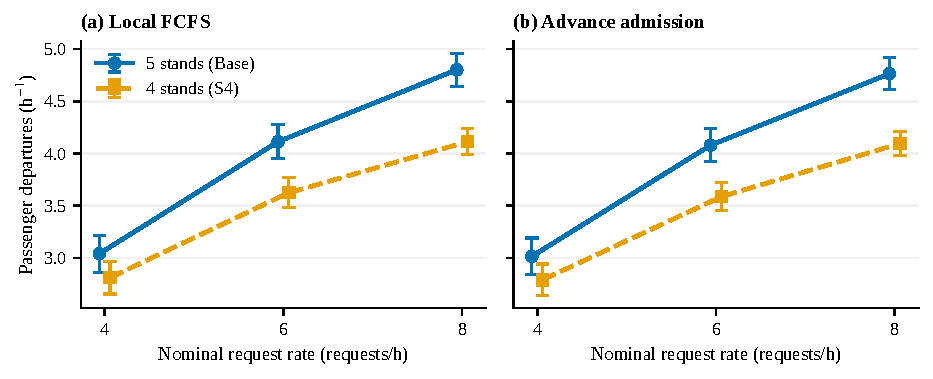
\includegraphics[width=0.9\linewidth]{fig_d4_vazao_demanda_en.pdf}
  \caption{Passenger departures per hour in the Base configuration by nominal request rate. Points
  are means of 30 independent replications and bars two-sided 95\% $t$ intervals. FCFS and
  advance admission share the same offered day within each replication.}
  \label{fig:flow}
\end{figure}

\begin{table}[htbp]
\centering\small
\caption{Request balance per replication in the Base configuration by demand (means of 30
replications). Refusals occur only under advance admission and diversions only under FCFS.
Coverage is departures with passengers over offered requests.}
\label{tab:demand}
\renewcommand{\arraystretch}{0.9}
\begin{tabular}{@{}lcccccc@{}}
\toprule
& \multicolumn{2}{c}{4 requests/h} & \multicolumn{2}{c}{6 requests/h} & \multicolumn{2}{c}{8 requests/h} \\
\cmidrule(lr){2-3}\cmidrule(lr){4-5}\cmidrule(l){6-7}
Indicator & FCFS & Adv. & FCFS & Adv. & FCFS & Adv. \\
\midrule
Offered requests & 28.70 & 28.70 & 43.77 & 43.77 & 57.97 & 57.97 \\
Refused or diverted & 1.60 & 1.80 & 6.77 & 7.23 & 14.23 & 14.63 \\
Empty departures & 0.53 & 0.53 & 0.87 & 0.83 & 1.10 & 1.13 \\
Pending at horizon & 2.23 & 2.23 & 3.23 & 3.07 & 4.23 & 4.10 \\
Passenger departures/h & 3.042 & 3.017 & 4.112 & 4.079 & 4.800 & 4.763 \\
Coverage of offered (\%) & 85.2 & 84.5 & 75.7 & 75.2 & 66.9 & 66.4 \\
Mean counter wait (s) & 94.8 & 89.6 & 154.8 & 137.7 & 222.2 & 186.4 \\
Counter waits within 180 s (\%) & 80.5 & 81.4 & 67.7 & 70.1 & 56.3 & 61.1 \\
\bottomrule
\end{tabular}
\end{table}

The throughput difference follows request selection. In the reference family, advance admission
refused 7.23 requests per replication at decision time, while FCFS diverted 6.77 when the
approach could not start within 300~s. Perfect information about arrivals and baggage changed
neither the throughput of advance admission (0.004 departures/h; $-0.015$ to $0.023$) nor its
refusals (0.03 per replication; $-0.17$ to $0.24$), so the residual difference does not stem from
forecasting passenger arrivals. Because a refusal removes the passengers of that request from the
terminal at decision time, the lower mean counter wait under advance admission (137.7 against
154.8~s) describes a smaller population and does not represent all offered requests.

\subsection{Stands, terminal waiting and group retention}

Table~\ref{tab:primary} and Figure~\ref{fig:contrasts} gather the primary contrasts and place them
beside the exploratory ones. The fifth stand added about 0.5 passenger departures/h under both
policies. With four stands, diversions under FCFS averaged 11.27 per replication against 6.77 in
Base, and refusals under advance admission 11.63 against 7.23. The physical occupation per stand
rose from 55.3\% to 60.4\% under FCFS. The archived event trace of seed 20001 shows the mechanism:
a request issued while four stands were held by cycles of about 38~min found no position within
300~s and diverted in S4, whereas in Base it landed on the fifth stand and departed.

\begin{table}[htbp]
\centering\small
\caption{Primary contrasts in the reference family: mean of within-replication differences and
95\% CI ($n=30$).}
\label{tab:primary}
\renewcommand{\arraystretch}{0.9}
\begin{tabular}{@{}llcc@{}}
\toprule
Contrast & Policy & Effect (95\% CI) & Unit \\
\midrule
Advance $-$ FCFS, Base & --- & $-0.033$ ($-0.066$; $-0.001$) & passenger departures/h \\
Base $-$ S4 & FCFS & 0.487 (0.439; 0.536) & passenger departures/h \\
Base $-$ S4 & Advance & 0.492 (0.440; 0.544) & passenger departures/h \\
B2 $-$ Base & FCFS & $-141.5$ ($-158.4$; $-124.7$) & counter wait, s \\
B2 $-$ Base & Advance & $-125.3$ ($-140.5$; $-110.1$) & counter wait, s \\
\bottomrule
\end{tabular}
\end{table}

\begin{figure}[htbp]
  \centering
  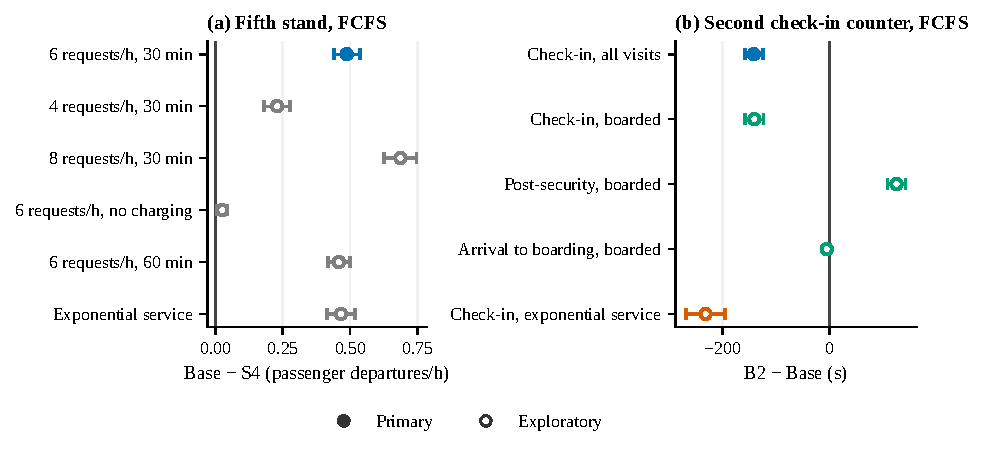
\includegraphics[width=\linewidth]{fig_d4_contrastes_en.pdf}
  \caption{Paired contrasts in the Base configuration and their sensitivity. Points are means of
  within-replication differences; bars are 95\% $t$ intervals ($n=30$). Filled markers are
  primary contrasts fixed before the runs; open markers are exploratory. In (b), counter waiting
  counts visits with an observed service start, and post-security waiting counts boarded
  passengers.}
  \label{fig:contrasts}
\end{figure}

The second counter lowered mean counter waiting from 154.8 to 13.3~s under FCFS and from 137.7 to
12.4~s under advance admission, over 2,529 and 2,608 FCFS visits in Base and B2 and 2,468 and 2,541
under advance admission. Against the IATA 180-s limit, compliance rose by 31.5 percentage points
under FCFS (27.7 to 35.3) and by 29.1 under advance admission (25.4 to 32.8), reaching 99.2\% in
both. The waiting did not leave the passenger's path (Figure~\ref{fig:wait}). B2 created mean waits
of 2.4~s at baggage and of 8.0 and 7.6~s at security, stations where Base forms no queue. The
post-security wait grew by 124.7~s under FCFS (107.9 to 141.5) and by 112.7~s under advance
admission (98.3 to 127.1). Since boarding waits for the aircraft, most of the waiting saved at the
counter moved to the lounge. The shift to downstream stations agrees with Feldhoff's explanation
that the counter's delay keeps later stations uncongested \cite{feldhoff2022}.

\begin{figure}[htbp]
  \centering
  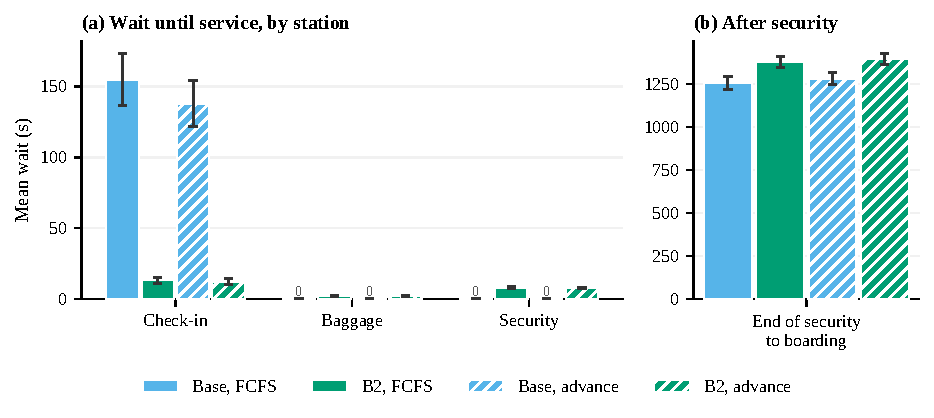
\includegraphics[width=\linewidth]{fig_d4_espera_en.pdf}
  \caption{Mean waiting in the reference family, Base and B2, under both policies. (a) Wait until
  service start at each station, over visits with an observed start; with one counter, baggage
  and security form no queue. (b) Wait from the end of security to the start of boarding, over
  boarded passengers, including 51.6~s of walking and aircraft access. Populations differ between
  panels and the means do not add up. Error bars: 95\% $t$ intervals ($n=30$).}
  \label{fig:wait}
\end{figure}

Relieving the counter also advanced group readiness. In Base, 9.2\% of the FCFS departures with
passengers were retained by their group, for 18.1~s on average; in B2, 2.3\% and 2.1~s. Under
advance admission the shares were 7.9\% in Base and 1.8\% in B2, with mean retentions of 13.3 and
1.7~s. These reductions did not translate into a comparable throughput gain (4.158 against 4.112
passenger departures/h under FCFS), because in the reference family the charging cycle and the
number of stands, not the readiness of the few retained groups, set the pace of departures.

\subsection{Sensitivity}

The exploratory families locate where each increment pays off (Figure~\ref{fig:contrasts}a and
Table~\ref{tab:sensitivity}). The stand gain grew with demand and with the time a stand is held:
it reached 0.688 departures/h at 8 requests/h and nearly vanished without charging. The counter
gain followed the opposite pattern across charging families. It peaked at $-268.5$~s without
charging, when almost no request was diverted (0.17 per replication under FCFS) and 2,902
passengers reached the counter in Base against 2,529 in the reference family. It shrank to
$-68.3$~s with 60-min charging. Advance admission stayed close to FCFS in every family, and perfect
information did not change its throughput with or without charging.

\begin{table}[htbp]
\centering\small
\caption{Exploratory sensitivity of the resource contrasts under FCFS (means and 95\% CI of
within-replication differences, $n=30$).}
\label{tab:sensitivity}
\renewcommand{\arraystretch}{0.9}
\begin{tabular}{@{}lccc@{}}
\toprule
Family & Base $-$ S4 & B2 $-$ Base & B2 $-$ Base \\
 & (passenger dep./h) & (counter wait, s) & (within 180 s, p.p.) \\
\midrule
4 requests/h, 30 min & 0.229 (0.180; 0.278) & $-87.7$ ($-104.3$; $-71.1$) & 19.2 (15.6; 22.9) \\
6 requests/h, 30 min & 0.487 (0.439; 0.536) & $-141.5$ ($-158.4$; $-124.7$) & 31.5 (27.7; 35.3) \\
8 requests/h, 30 min & 0.688 (0.628; 0.747) & $-202.9$ ($-228.4$; $-177.4$) & 42.0 (38.1; 45.8) \\
6 requests/h, no charging & 0.025 (0.006; 0.044) & $-268.5$ ($-328.1$; $-208.9$) & 43.5 (38.2; 48.8) \\
6 requests/h, 60 min & 0.458 (0.417; 0.500) & $-68.3$ ($-79.4$; $-57.2$) & 14.3 (11.4; 17.2) \\
\bottomrule
\end{tabular}
\end{table}

% ---------------------------------------------------------------------------------------
\section{Discussion}
\label{sec:discussion}

The two resource increments solve different problems. In the simulated regime, the stand is the
throughput intervention: it absorbs requests that would otherwise find every position held during
the 300-s window, which is the parking-induced arrival blocking discussed by Onat et al.\
\cite{onat2026buffer} and the parking-limited region found by Guerreiro et al.\
\cite{guerreiro2020}. Its value rises with demand and with charging time, and it adds almost
nothing when aircraft turn around without charging. The counter is the passenger-service
intervention: it brings counter waiting within the IATA limit for almost every passenger and cuts
group retention, but it moves most of the saved time to the lounge whenever boarding waits for a
charging aircraft. An operator who measures only counter queues would see the full benefit; one
who measures the time from processing to boarding would see a smaller one. The two measures are
complementary, and reporting both prevents a station-level improvement from being read as a
door-to-door one.

Advance admission and FCFS delivered nearly the same throughput. The policies differ less in
departures than in when passengers learn the outcome: a refused request is communicated at the
request time, whereas an FCFS diversion is communicated up to 300~s later. Halder and Gandhi \cite{halderGandhi2025} found that rule-based
departure sequencing outperformed FCFS in completed flights under fixed resources. Their rule
re-orders departures already in operation, while ours admits or refuses requests at arrival; the
two results together indicate that the sign of a scheduling benefit depends on the rule compared.
The execution rule matters as much as the admission rule. In an earlier version of this
experiment, the planned stand exit acted as a minimum time, and advance admission produced $-0.129$
departures/h, almost four times the present difference. Aircraft ready ahead of a pessimistic plan
were held on the stand, and their stands stayed reserved in the calendar.

The results compare designs within a synthetic scenario, and four of its features bound their
transfer to a real site. Most durations are expert estimates or author assumptions, and check-in
and security services are deterministic, which rules out security queues with one counter. The
uniform arrival shape is assumed. Each stand has its own charger and gate. The window starts empty
and lasts 8~h, and mean waits cover only visits whose service started. Request outcomes, empty
departures, censoring and denominators are reported next to every mean so that better service for
admitted passengers is not mistaken for better service of the offered demand.

% ---------------------------------------------------------------------------------------
\section{Conclusions}
\label{sec:conclusion}

We coupled per-station terminal queues, group readiness, charging and stand retention in a
verified discrete-event model of a single-TLOF vertiport and used paired replications to answer
two operational questions. A fifth stand raised passenger departures by about 0.5 per hour at
6 requests/h with 30-min charging, and its value grew with demand and charging time. A second
check-in counter cut mean counter waiting by 125--142~s, lifted compliance with the IATA limit to
99\% and reduced group retention, while most of the saved time reappeared in the lounge before
boarding. Advance admission matched FCFS in throughput within 0.033 departures/h once ready aircraft
were allowed to leave ahead of plan. For vertiport planners, the choice between a stand and a
counter is therefore a choice between departures and passenger service, and the charging time of
the fleet tells which one the next increment should buy. Station limits and the time from
processing to boarding should be reported together to show where that service is gained.

% ---------------------------------------------------------------------------------------
\section*{Declarations}
\textbf{Author contributions:} \pendente{to be completed by the authors (CRediT roles)}.
\textbf{Funding:} \pendente{to be completed by the authors}.
\textbf{Data and code availability:} archived inputs, seeds, results and scripts are versioned in
the project repository \pendente{repository access to be decided by the authors}.
\textbf{Use of AI tools:} drafting, analysis scripts and checks were assisted by AI coding agents
(Claude and Codex) using Scientific Agent Skills \cite{kassis2026skills}; all results come from
archived simulation outputs \pendente{wording to be confirmed by the authors under the venue
policy}.

\InputIfFileExists{referencias_aero.tex}{}{% Gerado por gerar_referencias.py a partir de references/references.bib.
% Não editar à mão.
\begin{thebibliography}{99}
\bibitem{guerreiro2020} N. M. Guerreiro, G. E. Hagen, J. M. Maddalon, R. W. Butler, AIAA AVIATION 2020 Forum, doi:\nolinkurl{10.2514/6.2020-2903}, (2020).
\bibitem{feldhoff2022} E. Feldhoff, AIAA AVIATION 2022 Forum, doi:\nolinkurl{10.2514/6.2022-3320}, (2022).
\bibitem{preisHornung2022} L. Preis, M. Hornung, Electronics, \textbf{11}, 1071, (2022).
\bibitem{escribanoMacias2023} J. Escribano Macias, C. Khalife, J. Slim, P. Angeloudis, Journal of Air Transport Management, \textbf{113}, 102486, (2023).
\bibitem{park2022} B. T. Park, H. Kim, S. H. Kim, International Journal of Aeronautical and Space Sciences, \textbf{23}, 1065 -- 1078, (2022).
\bibitem{rimjhaTrani2021} M. Rimjha, A. Trani, 2021 Integrated Communications Navigation and Surveillance Conference, 1 -- 14, (2021).
\bibitem{wille2026} E. Wille, J. Reichmuth, G. M. R. Borille, Journal of the Air Transport Research Society, \textbf{6}, 100109, (2026).
\bibitem{onat2026buffer} E. B. Onat, J.-L. Lupien, R. Sengupta, arXiv preprint 2609.37288v1, doi:\nolinkurl{10.48550/arXiv.2609.37288}, (2026).
\bibitem{kotwicz2024} M. T. Kotwicz Herniczek, B. J. German, L. Preis, Transportation Research Record, \textbf{2678}, 443 -- 469, (2024).
\bibitem{schweigerKnabeKorn2022} K. Schweiger, F. Knabe, B. Korn, Aerospace Science and Technology, \textbf{125}, 107144, (2022).
\bibitem{preisHornung2022heuristic} L. Preis, M. Hornung, Applied Sciences, \textbf{12}, 7260, (2022).
\bibitem{little1961} J. D. C. Little, Operations Research, \textbf{9}, 383 -- 387, (1961).
\bibitem{zhang2023capacity} H. Zhang, Y. Fei, J. Li, B. Li, H. Liu, Sustainability, \textbf{15}, 709, (2023).
\bibitem{kunchulia2021} Northeast UAS Airspace Integration Research Alliance, National Aeronautics and Space Administration, \url{https://ntrs.nasa.gov/citations/20210016168}, (2021).
\bibitem{saxena2025vertiminal} R. R. Saxena, T. V. Prabhakar, J. Kuri, M. Yadav, arXiv preprint arXiv:2408.01152v3, \url{https://arxiv.org/abs/2408.01152}, (2025).
\bibitem{preis2023} L. Preis, CEAS Aeronautical Journal, \textbf{14}, 353 -- 368, (2023).
\bibitem{bennaceur2022} M. Bennaceur, R. Delmas, Y. Hamadi, Transportation Research Part C: Emerging Technologies, \textbf{136}, 103519, (2022).
\bibitem{easa2022ptsvptdsn} European Union Aviation Safety Agency, PTS-VPT-DSN, \url{https://www.easa.europa.eu/sites/default/files/dfu/PTS-VPT-DSN.pdf}, (2022).
\bibitem{vascikHansman2019} P. D. Vascik, R. J. Hansman, AIAA Scitech 2019 Forum, doi:\nolinkurl{10.2514/6.2019-0526}, (2019).
\bibitem{wille2024icas} E. Wille, 34th Congress of the International Council of the Aeronautical Sciences, \url{https://www.icas.org/icas_archive/icas2024/data/papers/icas2024_0155_paper.pdf}, (2024).
\bibitem{marintseva2014} K. Marintseva, Proceedings of the National Aviation University, \textbf{59}, 97 -- 104, (2014).
\bibitem{janssen2020security} S. A. M. Janssen, R. van der Sommen, A. Dilweg, A. Sharpanskykh, Aerospace, \textbf{7}, 69, (2020).
\bibitem{feldhoffSoaresRoque2021} E. Feldhoff, G. Soares Roque, CEAS Aeronautical Journal, \textbf{12}, 821 -- 833, (2021).
\bibitem{postorino2019} M. N. Postorino, L. Mantecchini, C. Malandri, F. Paganelli, Transportation Research Procedia, \textbf{37}, 338 -- 345, (2019).
\bibitem{vojtek2021} N. Vojtek, B. Petrovi{\'c}, P. Milo{\v s}evi{\'c}, Technical Gazette, \textbf{28}, 123 -- 134, (2021).
\bibitem{law2023design} A. M. Law, Proceedings of the 2023 Winter Simulation Conference, \url{https://www.informs-sim.org/wsc23papers/124.pdf}, (2023).
\bibitem{halderGandhi2025} A. Halder, F. Gandhi, AIAA AVIATION FORUM AND ASCEND 2025, doi:\nolinkurl{10.2514/6.2025-3308}, (2025).
\bibitem{kassis2026skills} T. Kassis, V. Agarwal, Y. He, D. Patel, A. M. Brueckner, arXiv preprint 2609.00065, doi:\nolinkurl{10.48550/arXiv.2609.00065}, (2026).
\end{thebibliography}
}

\section*{Biography}
L. H. Tozi is a master's student at Instituto Tecnológico de Aeronáutica (ITA), Brazil.
\pendente{to be completed by the author; up to 150 words}

\end{document}
